\documentclass[UTF8]{ctexart}
% \usepackage{array}
% https://blog.csdn.net/tianzong2019/article/details/106521432
\usepackage{graphicx} %插入图片 需要用到graphicx 宏包
\usepackage{listings} %插入代码
\usepackage{xcolor}   %代码高亮
\usepackage{multicol} % 分栏目
\usepackage{geometry} %页面设置需要添加这个宏
\geometry{left=1.2cm,right=1.2cm,top=1.2cm,bottom=1.2cm}

%设置代码的格式
\lstset{
 columns=fixed,
 numbers=left,                                        % 在左侧显示行号
 numberstyle=\tiny\color{gray},                       % 设定行号格式
 frame=none,                                          % 不显示背景边框
 backgroundcolor=\color[RGB]{245,245,244},            % 设定背景颜色
 keywordstyle=\color[RGB]{40,40,255},                 % 设定关键字颜色
 numberstyle=\footnotesize\color{darkgray},
 commentstyle=\it\color[RGB]{0,96,96},                % 设置代码注释的格式
 stringstyle=\rmfamily\slshape\color[RGB]{128,0,0},   % 设置字符串格式
 showstringspaces=false,                              % 不显示字符串中的空格
%  language=c++,                                        % 设置语言
}


\title{你好,World!}
\author{Dingxin Liu}
\date{\today}

% 文档开始
\begin{document}

% 纸扎标题
\begin{titlepage}
    \maketitle %将title 编译进来
    \centering
    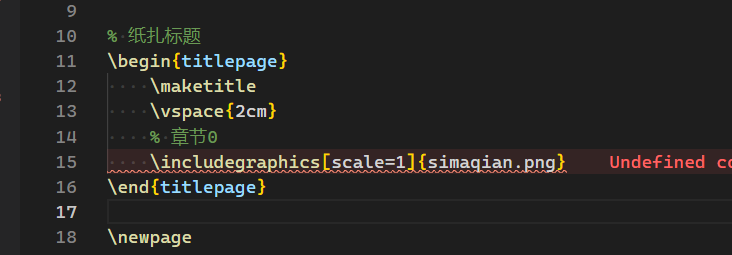
\includegraphics[scale=1.5]{simaqian.png}

\end{titlepage}


\newpage

\begin{abstract}
    abstract。这是摘要
    \begin{quote}
        \begin{center}
            {\kaishu
                床前明月光,\newline
                疑是地上霜。\newline
                举头望明月,\newline
                低头思故乡。\newline}
        \end{center}
    \end{quote}
\end{abstract}

\tableofcontents
\newpage


\section{页面设置}
\centering
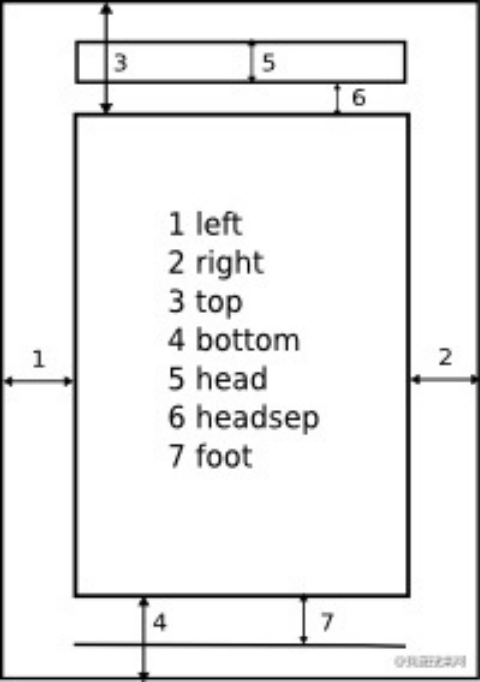
\includegraphics[scale=1]{geometry.png}
\newline

页面设置需要引用一个宏包

\begin{lstlisting}[language=tex]
    \usepackage{geometry} % 页面设置
    \geometry{left=2.5cm,right=2.5cm,top=2.5cm,bottom=2.5cm}
\end{lstlisting}

% 章节0
\section{如何使用Latex 编写漂亮的文章呢}
% 正文
中国在East Asia.

% 章节1
\subsection{Hello Beijing}
北京是capital of China.
% 章节1.1
\subsubsection{Hello Dongcheng District}
\subsubsection{Hello Dongcheng District}

%  paragraph
\paragraph{Tian'anmen Square}

is in the center of Beijing
% paragraph 段落
\subparagraph{Chairman Mao    is in the center of 天安门广场。subparagraph}



% 章节1
\subsection{Hello 山东}
% paragraph
\paragraph{山东大学} is one of the best university in 山东。


\newpage

\section{新增一个page 以及新增一个章节}
章节描述
\paragraph{\LaTeX{}的使用方法paragraph}

paragraph 下面的文字
\subparagraph{\LaTeX{} 的使用方法subparagraph}
subparagraph 下面的文字
\paragraph{\LaTeX{} 的使用方法paragraph}
subparagraph 下面的文字
\subparagraph{\LaTeX{} 的使用方法subparagraph}
subparagraph 下面的文字

\section{新增一个page2 以及新增一个章节}

\begin{lstlisting}[language=xml]



\end{lstlisting}


\begin{lstlisting}[language=c]
    void mian(int argl,string[] args){
        for(int i = 0;i<argl;)
            cout<<args[i]<<cendl;
    }
\end{lstlisting}



\begin{multicols}{2}  %分2栏
    孟达,1953年1月2日出生。1973年报考了第三期香港无线电视艺员培训班,同学包括周润发、林岭东等,他的成绩一直都名列前五名。1979年,吴孟达演了《楚留香传奇》里的男二号“胡铁花”,而开始受到注意。
\end{multicols}
\begin{multicols}{2}

    光和周星驰合作的片子就有《整蛊专家》《赌圣》《赌侠》《上海滩赌圣》《逃学威龙》《鹿鼎记》《逃学威龙2》《武状元苏乞儿》《审死官》《九品芝麻官》《食神》《喜剧之王》《少林足球》《行运一条龙》等。
\end{multicols}
\end{document}